%%%%%%%%%%%%%%%%%%%%%%%%%%%%%%%%%%%%%%%%%%%%%%%%%%%%%%%%%%%%%%%%%%%%
%PLANTILLA DE INFORMES V 1.1
%
% REQUISITO: IMPORTE EL LOGO DE LA USM CON EL NOMBRE "logousm.png"
% IMPORTE IMAGENES DE MODULOS, EXTRAER DEL WORD
%
% Material de referencia de proposito general:
% https://users.dcc.uchile.cl/~jbarrios/latex/
% http://mate.dm.uba.ar/~pdenapo/tutorial-latex/node2.html
% http://tiburondealambre.blogspot.cl/2012/01/referencias-imagenes-y-tablas-en-latex.html
% BIBLIOGRAFIA: http://logistica.fime.uanl.mx/miguel/docs/BibTeX.pdf
%
% Tratar ecuaciones en latex(muy util):
% https://ondiz.github.io/cursoLatex/Contenido/05.Ecuaciones.html
%
% detector de cosas dibujadas latex: http://detexify.kirelabs.org/classify.html
%
%%%%%%%%%%%%%%%%%%%%%%%%%%%%%%%%%%%%%%%%%%%%%%%%%%%%%%%%%%%%%%%%%%%%%%%

%----------------------PAQUETES---------------------------%
% No es necesario tocar nada de esto

\documentclass[12pt,a4paper]{article} % tipo de documento, formato

\usepackage[utf8]{inputenc}    % con tildes
\usepackage[spanish]{babel}    % arreglar problemas

\usepackage[framed,numbered,final]{mcode} %%MATLAB
\usepackage{listings}   % Permite incorporar código con d


\usepackage{graphicx} % paquete de tratado de imagenes/figuras
\usepackage{tipa} % para <
\usepackage{amssymb} % para >=

% paquete extra para ocupar [H] (obliga a que la imagen con graphicx
% se quede donde se realizó el llamado)
\usepackage{float}

% CARGAMOS 3 PAQUETES
% (AMS Math), que mejora el comportamiento y el aspecto de las ecuaciones. 
% Nos permite, por ejemplo, añadir un asterisco en el entorno equation para crear
% ecuaciones sin numerar.
%(AMS Theorem), que define los entornos teorema y demostración.
%(AMS Symbol), que carga a su vez amsfonts e incluye una colección 
%de símbolos matemáticos.
\usepackage{amsmath, amsthm, amssymb} 

\usepackage{enumerate} %permite enumerar de varias formas

\usepackage{multirow, array} % para las tablas

% construccion de un nuevo comando
\usepackage{lipsum}% http://ctan.org/pkg/lipsum
\usepackage{xcolor}% http://ctan.org/pkg/xcolor
\usepackage{xparse}% http://ctan.org/pkg/xparse
\NewDocumentCommand{\myrule}{O{1pt} O{2pt} O{black}}{%
  \par\nobreak % don't break a page here
  \kern\the\prevdepth % don't take into account the depth of the preceding line
  \kern#2 % space before the rule
  {\color{#3}\hrule height #1 width\hsize} % the rule
  \kern#2 % space after the rule
  \nointerlineskip % no additional space after the rule
}

%acomoda margenes y tipografia para que quede mas bonito
\usepackage{geometry}
\geometry{
	paper=a4paper, % Change to letterpaper for US letter
	inner=3cm, % Inner margin
	outer=3cm, % Outer margin
	bindingoffset=.5cm, % Binding offset
	top=2cm, % Top margin
	bottom=2cm, % Bottom margin
	%showframe, % Uncomment to show how the type block is set on the page
}


%---------PORTADA, TABLA DE CONTENIOS Y FIGURAS--------------%
%Esto será la portada. Solo hay que cambiar los textos
\begin{document}

\begin{titlepage}
\begin{center}
\textbf{\LARGE Universidad Técnica Federico Santa}\\[0.25cm]
\textbf{\LARGE María}\\[0.5cm]
\textbf{\large DEPARTAMENTO DE INGENIERIA ELECTRÓNICA}\\[0.2cm]
\vspace{20pt}

\includegraphics{logousm.png}\\[1cm]

\par
\vspace{15pt}
\textbf{\Large ELO 314 - Laboratorio de procesamiento Digital de Senales}\\
\vspace{15pt}
\myrule[1pt][7pt]
\textbf{\LARGE  Señales de Audio en MatLab}\\[0.25cm]
\vspace{15pt}
\textbf{\large  }\\
\myrule[1pt][7pt]
\vspace{55pt}
\textbf{\large Estudiante \hspace{75pt} ROL}\\
    \hspace{0pt}Rodrigo Graves\hspace{75pt} 201621009-1 \\
     Ricardo Mardones      \hspace{60pt} 201621036-9 \\
   


\vspace{30pt}
\textbf{\large Paralelo: \hspace{30pt} 1}\\

\vspace{35pt}
\textbf {\large Profesor}\\[0.2cm]
\Large { Gonzalo Carrasco}\\[0.1cm]
\textbf {\large Ayudante}\\[0.2cm]
\Large {Jaime Guzman}\\[0.1cm]
\end{center}

\par
\vfill
\begin{center}
\textbf{Fecha : \today}\\
\end{center}

\end{titlepage}


%-------------Lista de figuras y tablas----------%
\tableofcontents % Hace el índice de contenidos. Latex organiza todo solito
\clearpage

\listoffigures %lista de figuras
\clearpage

\listoftables
\clearpage


\section{Archivos de Audio y Visualización}
\subsection{Extracción y Guardado de Segmentos de Audio}

Para esta sección se utiliza el script de MATLAB \texttt{rp1.m}, el cual se adjunta en la entrega.

Se carga el archivo \textit{besh.wav} como vector en MATLAB y se extraen las porciones de la vocal /$\epsilon$/ y la fricativa /sh/. En la figura \ref{fig:p11_extraccion} se muestra el gráfico de la señal \textit{besh.wav} y extracción de las secciones de audio de interés.

\begin{figure}[H]
    \centering
    \includegraphics[width = .8\linewidth]{Figuras/p11_extracción.eps}
    \caption{Audio \textit{besh.wav} y extracción de la vocal /$\epsilon$/ y fricativa /sh/.}
    \label{fig:p11_extraccion}
\end{figure}

Se guarda además el segmento de audio correspondiente a la vocal /$\epsilon$/ como \textit{Lab2p1\_vocal.wav} y se adjunta a la entrega.

\subsection{Función en MATLAB para la selección gráfica de un segmento de Audio}

Se escribe la función en MATLAB \texttt{select\_wav} con la cual se selecciona con el mouse un segmento de una señal, se copia dicho segmento en un vector y se guarda en un archivo de audio. La función descrita se muestra a continuación:

\lstinputlisting[language = octave]{Code/select_wav.m}

Se utiliza la función para extraer el segmento de la vocal /$\epsilon$/, quedando guardado en el archivo \textit{lab2p1\_segmento vocal}. Se adjunta dicho archivo a la entrega.
\clearpage

\section{Efectos de Audio}
\subsection{Implementación de Overdrive en MATLAB}

%comentar que script se utiliza

Se implementa en MATLAB un overdrive simple dado por la siguiente expresón:
\begin{align}
    x' &= G_i x \\ 
    y' &= \begin{cases}
    \beta x' + \text{sign}(x')(1-\beta) \alpha \hspace{2 cm} &\text{si }\abs{x'} \geq \alpha\\
    x' &\text{si }\abs{x'} < \alpha
    \end{cases}\\
    y &= G_o y'
\end{align}

La función implementada se muestra a continuación:

\lstinputlisting[language = octave]{Code/overdrive.m}

Posteriormente se aplica dicha función al archivo de audio \texttt{gtr\_jazz.wav} obteniendo el audio \texttt{gtr-ov\_a02b005Gi1Go1.wav} el cual utiliza $\alpha = 0.2, \beta = 0.05$ y $G_i = G_o = 1$. Se adjunta el audio resultante a la entrega. 
\\
Con respecto a la percepción auditiva, se pecibe una clara distorsión en el sonido. Lo anterior se le atribuye a que la función overdrive es no lineal por lo tanto cambia el contenido en frecuencias de la señal.
\\
\newline
Se pide aplicar el efecto a una señal de audio adecuada para una comparación visual de lo que hace el efecto sobre la señal. Se considera \texttt{gtr\_jazz.wav} un buen audio para lo anterior, pues debido a sus claros cambios de intensidad en el sonido se pasa de zona lineal a no lineal con frecuencia.

En la figura \ref{fig:p211} se muestra el audio \textit{gtr-.wav} original y luego de aplicar overdrive. Se nota claramente que la distorsión cumple su cometido, añadiendo cambios bruscos en la señal, lo cual puede interpretarse como que se agregaron componentes de alta frecuencia.

\begin{figure}[H]
    \centering
    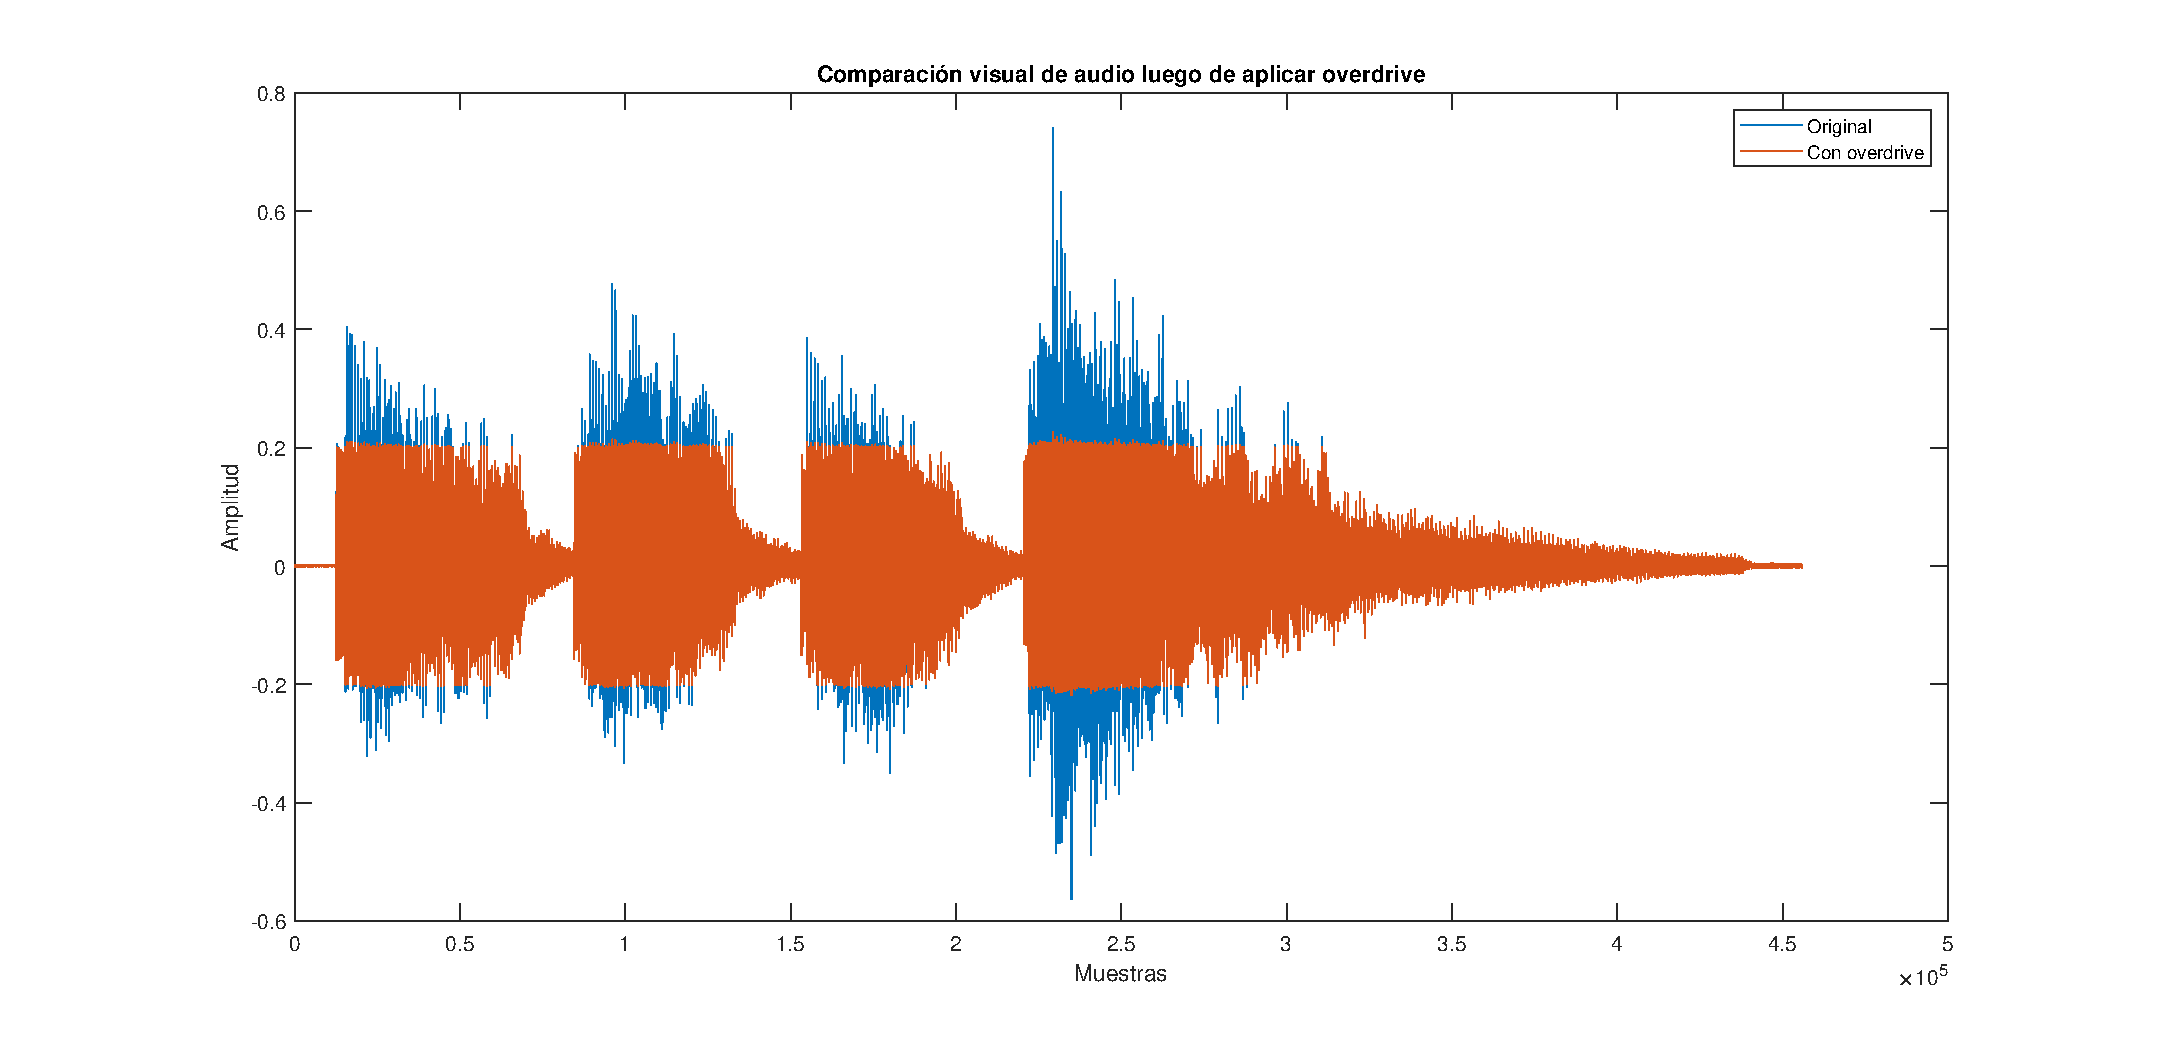
\includegraphics[width = .8\linewidth]{Figuras/p211_comparacion-overdrive.eps}
    \caption{Audio \textit{gtr-.wav} original y luego de aplicar overdrive.}
    \label{fig:p211}
\end{figure}

Posteriormente se analiza que ocurre al variar los parámetros de la función, tomando $\alpha=0.1$ y $G_i = 3$. La relación salida/entra de este overdrive y el original se muestra en la figura \ref{fig:p212}.

\begin{figure}[H]
    \centering
    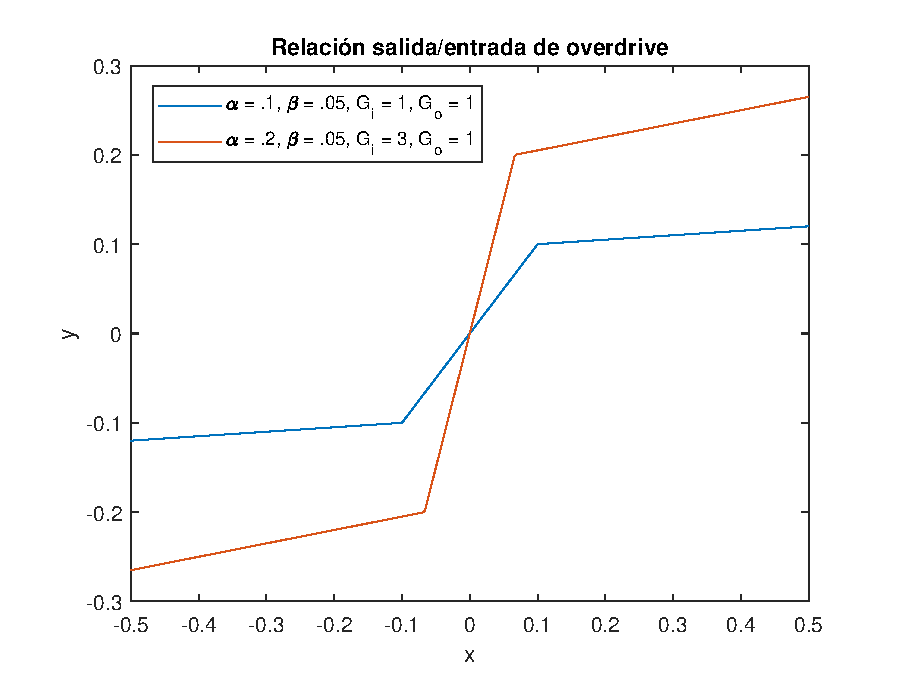
\includegraphics[width = .8\linewidth]{Figuras/p212_relacion-overdrive.eps}
    \caption{Relación Salida/Entrada de overdrive con distintos parámetros.}
    \label{fig:p212}
\end{figure}

A partir de la figura \ref{fig:p212} se aprecia que el overdrive con los nuevos parámetros genera una señal con menos energía que el anterior, pues cada punto azul es menor en magnitud a su punto rojo correspondiente para algún valor $x$ de entrada. Lo anterior podría corregirse variando $G_o$. Por otro lado vemos que con la nueva combinación de parámetros el cambio de pendiente es aparentemente menos abrupto, por lo que se esperaría una percepción auditiva menor en el overdrive. Además, la zona lineal aumenta, lo cual es otra razón para que la percepción auditiva de la distorsión producto al overdrive sea menor.

Los parámetros del modelo de overdrive utilizado pueden interpretarse de la siguiente forma:
\begin{itemize}
    \item $G_i$: Ganancia de entrada. la cual sirve para balancear que la señal $x'$ ''se mueva'' por los intervalos de no linealidad. Si $G_i$ es muy bajo no habrá distorsión. 
    \item $\alpha$: Umbral de no linealidad. Si $\alpha$ es muy alto no hay distorsión pues $x$ estaría en zona lineal. De la misma forma si $\alpha$ es muy pequeño no se aprecia distorsión.
    \item $\beta$: Relacionado a que tan abrupto es el cambio de pendiente en el módulo no lineal (ecuación de $y'$). Afecta a la percepción de la distorsión. 
    \item: $G_o$: Ganancia de salida. Está relacionada con el ''volumen'' de la señal de salida. No genera distorsión.
\end{itemize}

\subsection{Implementación de un Delay Multi-Tap}

Una implementación de un delay multitap corresponde a la siguiente expresión
\begin{equation}
    y[n] = \sum_{k=1}^N b(k)x[n-k\cdot M]
\end{equation}

Donde:
\begin{itemize}
    \item $x$: Señal de entrada
    \item $N$: Número de etapas de retardo.
    \item $M$: Número de muestras equivalentes a la longitud de cada retardo. Dado $T$ un retardo por etapa deseado en s y una $T_s$ periodo de muestreo, $M$ puede obtenerse como:
    $$M = \dfrac{T}{T_s}$$
    \item $b(k)$: Ganancia de la $k$-ésima etapa.
\end{itemize}

En primer lugar se solicita aplicar un delay multi-tap de 4 etapas ($N$) de longitud 125 ms ($T$) y ganancia constante $b(k) = 0.35$ al archivo \textit{gtr-jazz.wav}. 

Auditivamente se nota que el efecto de repetición de la señal a modo de ''eco'', sin embargo, el hecho de que $b(k)$ se mantenga constante hace que el sonido sea antinatural. El archivo de audio obtenido corresponde a \textit{gtr-jazz\_delay-multitap.wav}, el cual se adjunta en la entrega

La función creada para implementar el delay multi-tap en MATLAB se muestra a continuación:

\lstinputlisting[language = octave]{Code/delay_multitap.m}

Se decide que \textit{gtr-jazz.wav} es una buena señal para mostrar el efecto del delay muli-tap debido a los claros ecos escuchados en la señal de audio resultante. El gráfico resultante se muestra en la figura \ref{fig:p221}. 

\begin{figure}[H]
    \centering
    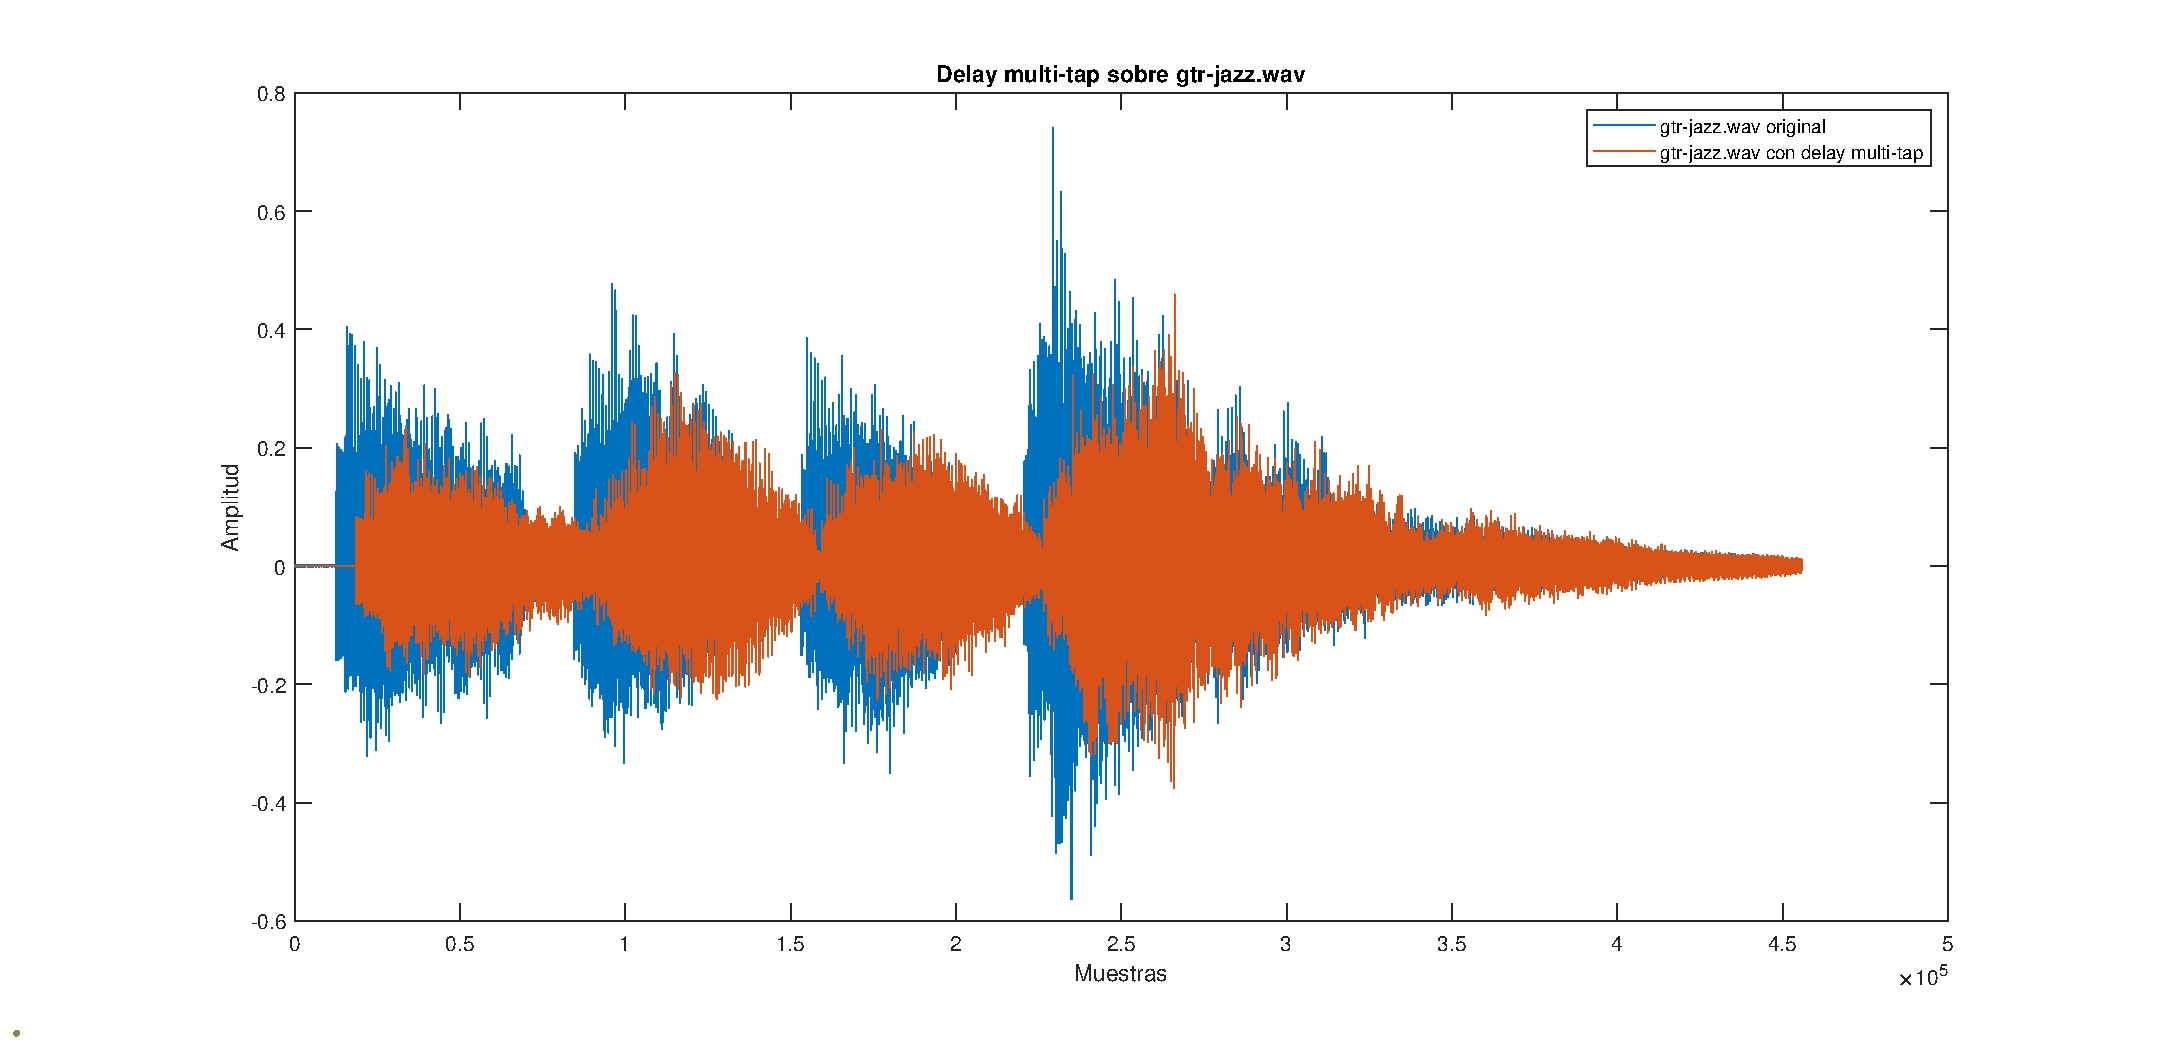
\includegraphics[width = .8\linewidth]{Figuras/p221_comparacion-delay.eps}
    \caption{Audio \textit{gtr-jazz.wav} original y luego de aplicar delay multi-tap.}
    \label{fig:p221}
\end{figure}

Curiosamente no se logra apreciar el eco de forma visual, pero si el efecto de filtro pasabajos que tiene un filtro de media móvil de ganancias constantes. Lo anterior se le atribuye a que el tiempo de retardo es muy bajo para la duración de los ''segmentos'' de la señal (arpegios).

Posteriormente se cambia $N=10$, $T = 250$ ms y $b(k) = 0.35^k$ y se vuelve a aplicar el efecto a \textit{gtr-jazz.wav}, obteniendo \textit{gtr-jazz\_delay-multitap2.wav}, el cual se adjunta en la entrega. Auditivamente se siente un decaimiento mucho más natural del eco. Una comparación gráfica se muestra en la figura \ref{fig:p222} , siendo notoria una mayor atenuación en la señal que con ganancias constantes.

\begin{figure}[H]
    \centering
    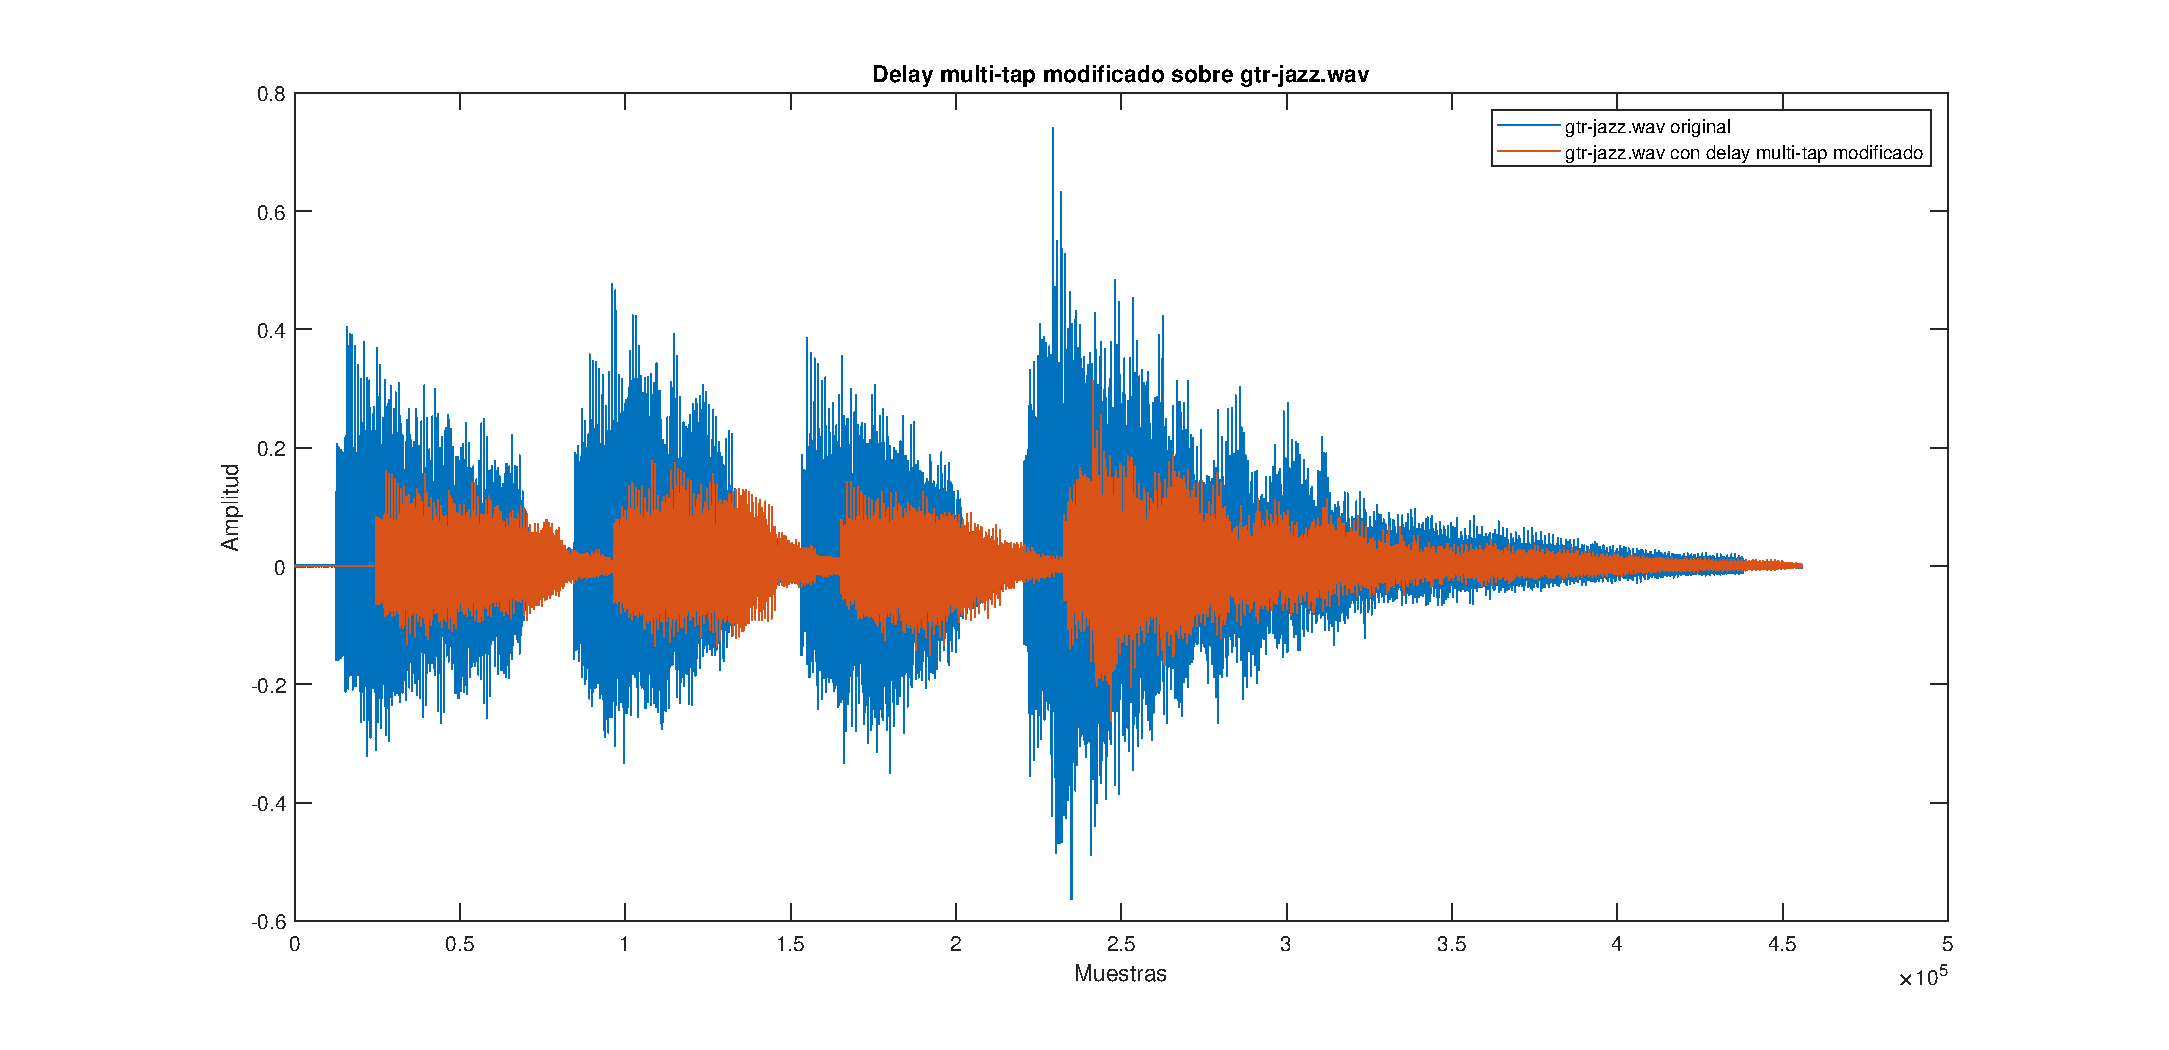
\includegraphics[width = .8\linewidth]{Figuras/p222_comparacion-delay.eps}
    \caption{Comparación entre audio \textit{gtr-jazz.wav} original y luego de aplicar delay multi-tap con ganancia $b(k) = 0.35^k$.}
    \label{fig:p222}
\end{figure}

Finalmente se modificó la frecuencia de muestreo en el audio \textit{gtr-jazz.wav} a 16 kHz usando el comando \texttt{resample}. El audio a la nueva frecuencia de muestreo se guardo en el archivo \textit{gtr-jazz\_resample-16.wav} el cual se adjunta con la entrega. Auditivamente no se escucha mayor diferencia con el audio original. Los parámetros elegidos para lograr el mismo efecto anterior corresponden a:
\begin{itemize}
    \item $N$: Se mantiene en 10, pues las etapas no cambian.
    \item $M$: Al cambiar la frecuencia de muestreo este cambia. Como la frecuencia de muestro original (48 kHz), es el triple de la nueva (16 kHz), ahora M corresponde a un tercio de las muestras anteriores.
    \item $b(k)$: Se mantiene pues no se cambia la ganancia por etapa.
\end{itemize}

El audio obtenido al aplicar los nuevos parámetros de delay sobre la señal a la nueva tasa de muestre se guarda en el archivo \textit{gtr-jazz\_resample-16\_delay.wav}, el cual se adjunta en la entrega. No se perciben diferencias auditivas notorias con el audio a 48 kHz.

Con respecto a las ventajas y desventajas de aplicar resample se tiene:
\begin{itemize}
    \item Ventajas: Menor tiempo de cálculo de la salida del filtro. En aplicaciones que tengan algún requisito de tiempo máximo para procesamiento puede ser útil.
    
    \item Desventajas: El cambio de frecuencia de muestreo puede provocar perdida de contenido espectral de interés.
\end{itemize}



\clearpage

\section{Buffers Lineales y Circulares en Lenguaje C}
\subsection{Buffer lineal}


\begin{enumerate}
    \item 

Para lograr una linea de retardo se implementa un buffer lineal en lenguaje C, integrado a MATLAB mediante el uso de \textit{s-function}.

El siguiente código muestra la función en lenguaje C que implementa el buffer.

    \begin{lstlisting}
    
#define N (32000)
double retardo_lineal(double input) {
	// Buffer lineal
	static double buffer[N];
    
    //Inicializacion del buffer
	static int flag = 1;
    
	if (flag == 1) {
		for (int i = 0; i < N; i++) {
			buffer[i] = 0;
		}
		flag = 0;
	}

	double output = buffer[N - 1];

	for (int idx = N - 1 ; idx >= 1; idx--) {
		buffer[idx] = buffer[idx -1];
	}
	buffer[0] = input;
	return output;
}

    \end{lstlisting}
    
    Donde la entrada a la función es una muestra actual n de la señal que se desea retardar, dato que se guarda en el buffer de N elementos, mientras que la salida retornada por la función corresponde a la primera posición del buffer, es decir el dato guardado  n - N.
    
    
    
    
    Para verificar el correcto funcionamiento de este retardo lineal implementado se escoge el archivo de audio \textit{sonidos\_de\_voz\_16\_8.wav} ya que por la manera en la que está distribuida la información  en el tiempo en este archivo (viendo la forma de onda a graficar los datos del arhcivo) un retardo en un mensaje hablado es significativamente notorio. En este punto es necesario comentar la relación que existe entre el \textbf{tiempo de retardo}  y la frecuencia de muestreo \textbf{Fs} asociado a las señales a trabajar, el inverso de esta frecuencia corresponde al periodo de muestreo , que al ser multiplicado por la cantidad de muestras que se desean almacenar en el buffer se obtiene el tiempo total de retardo provocado en la señal. 
    
    
    La frecuencia de muestreo de la señal escogida es de  $8~kHz$, por lo que con un N de 32000 muestras se debiera obtener un retardo de $4~s$ como se muestra a continuación
    
    $$T_{retardo} = \frac{1}{Fs}\cdot N = \frac{1}{8 ~kHz}\cdot 32000 = 4~s$$
    
     Se crean los bloques necesarios para hacer uso de la \textit{s-Function} creada, importar el archivo de audio y un scope para poder observar y comparar las señales obteniendo de esta forma las gráficas presentes en la figura \ref{retardo_lineal}  
    
    Cabe destacar que si bien la guía propone un retardo de $N = 100$ , debido a la frecuencia de muestreo que posee el archivo de audio esta cifra provocaría un retardo despreciable por lo que se optó por un  valor de $N = 32000$, tal como se mencionó antes.
    
    \begin{figure}[H]
        \centering
        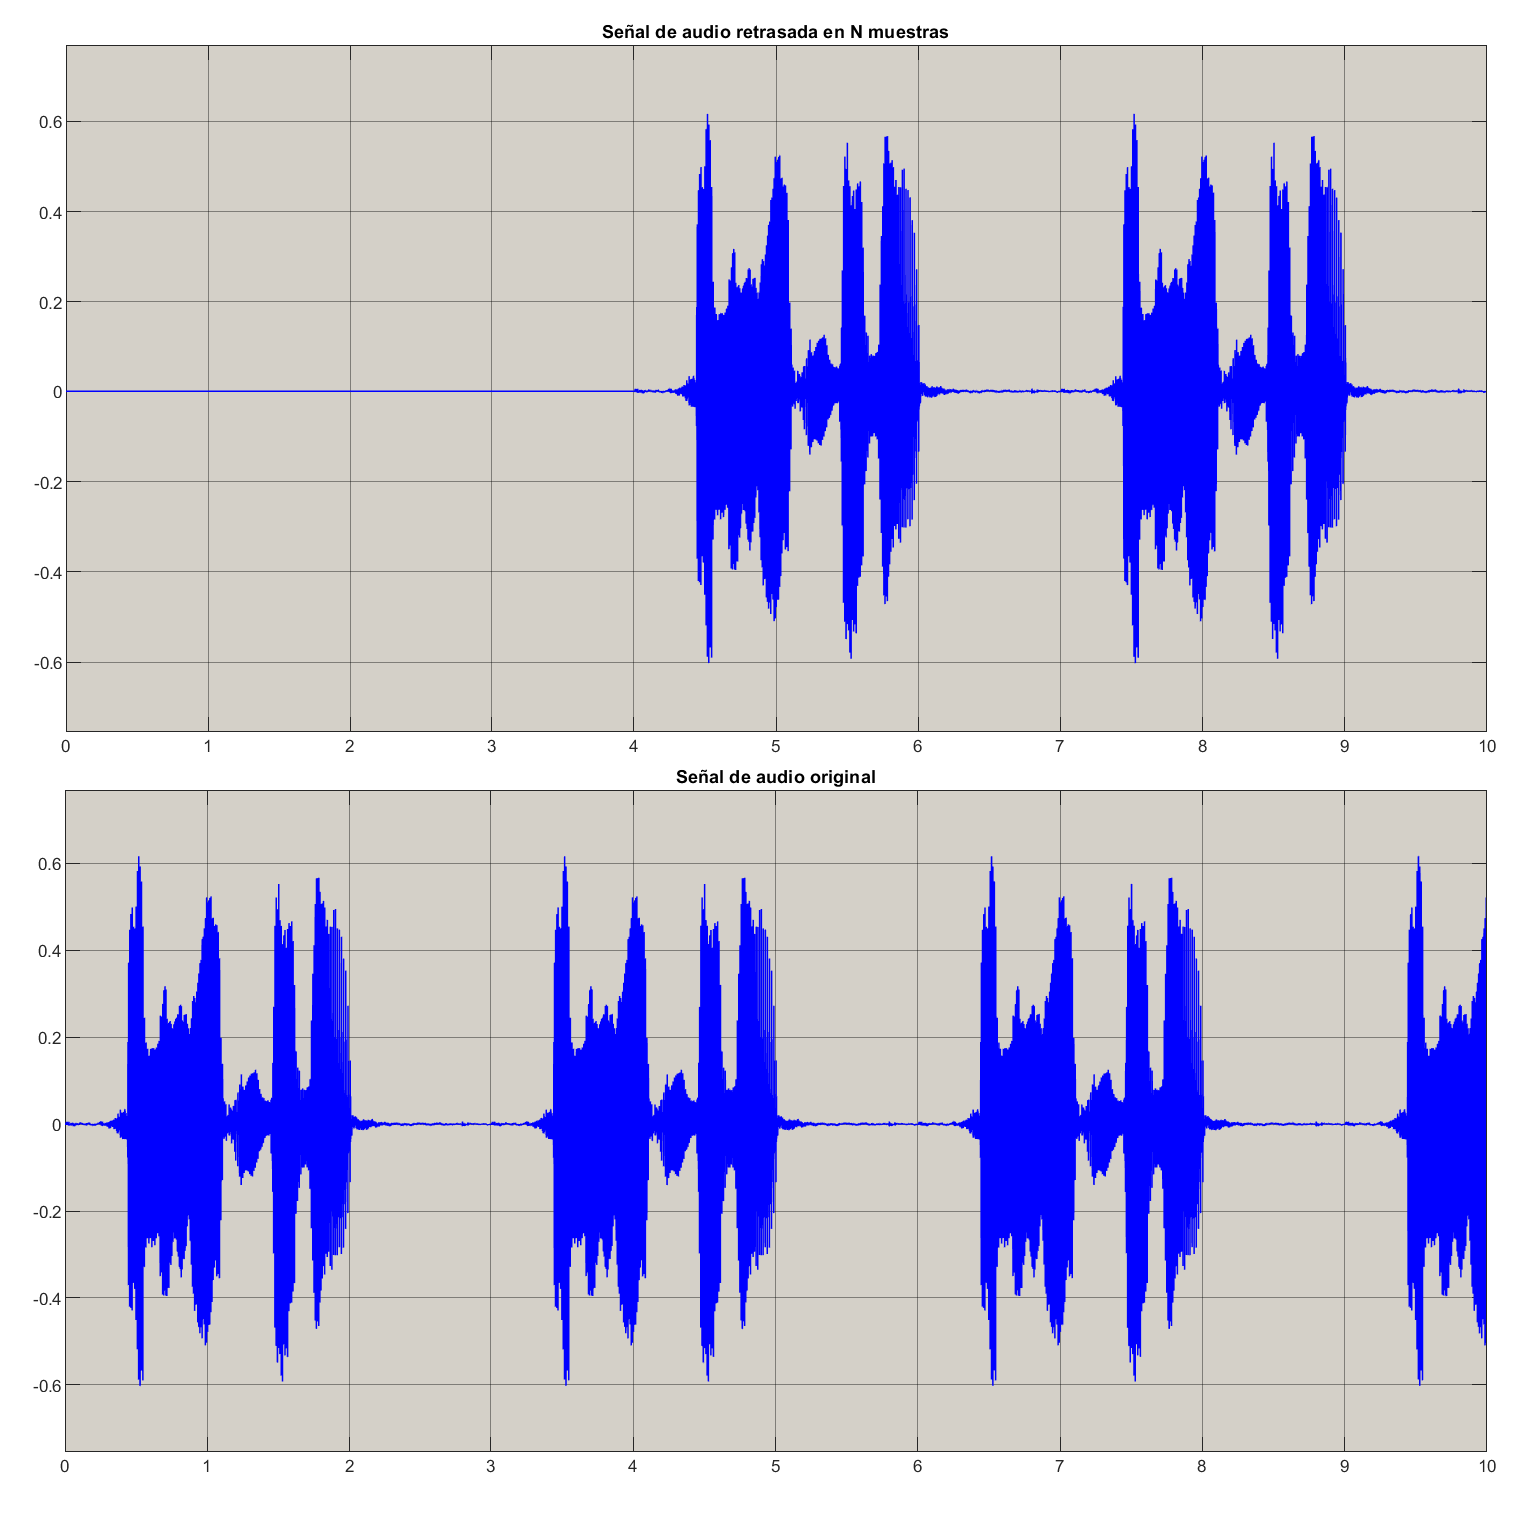
\includegraphics[scale = 0.5]{Figuras/p31_retardo_lineal.eps}
        \caption{Gráfica del resultado de aplicar el retardo lineal implementado a una señal de audio.}
        \label{retardo_lineal}
    \end{figure}
    
    En la figura anterior se puede ver que tal como se esperaba el buffer lineal implementado provoca un retardo de $4~s$ respecto de la señal de audio original desplazándola en 32000 muestras  hacia la derecha.
    
    \item
    
    De la misma manera que en el apartado anterior, se implementa una linea de retardo usando código en lenguaje C pero esta vez haciendo uso de un \textbf{buffer circular} en tiempo real, el código de implementación es el siguiente
    
    \newpage
    \begin{lstlisting}
    
    #define n (32000)
    double retardo_circular(double input) {
    
    
    
    static double buffer[n]; //Crea buffer tamaño n
    	
    //inicialica el "puntero" idx en la ultima posicion
    static  int idx = n-1;  
    
    //Bloque para inicializar el buffer con ceros
    static int flag = 1;
    
    if (flag == 1) 
    {
    	for (int i = 0; i < n; i++) 
    	{
    		buffer[i] = 0;
    	}
        flag = 0;
    } 
    //Fin inicializacion del Buffer
    
    double output = buffer[idx]; //Lee dato del Buffer
    buffer[idx] = input;  //Actualiza el dato en posicion idx
    idx = ((idx+1)%n); //Actualiza posicion idx
    
    
    return (output);
    }

    \end{lstlisting} 
    
    Al graficar la señal original y la que sufrió el retardo debido usando buffer circular son practicamente idénticas  a las gráficas obtenidas con el buffer de tipo lineal ya que ambas implementaciones cumplen el objetivo que es provocar un retardo.
    
\item Para comparar la eficiencia de ambos métodos para retardo implementados,  usando el modo \textit{PROFILE} de simulink se estudian los tiempos de ejecución de la simulación que requieren ambas \textit{s-Function} (la asociada a buffer llineal y a buffer circular respectivamente). De este modo se obtuvieron los datos que se presentan en los cuadros \ref{lin_tabl} y \ref{circ_tabl}




\begin{table}[H]
        \centering
        \begin{tabular}{|c|c|c|c|c|c|c|}
        \hline
 N  & Scope & From multimedia file & s-Function & Simulacion & Total \\
 \hline
 20 &0,042	&0,091	&0,019	&0,563	&0,612 \\
 \hline
 200 & 0,044 &	0,091	&0,024&	0,488&	0,647 \\
 \hline
 2000 &0,045 &	0,099	&0,079&	0,482&	0,705\\
 \hline

 20000 & 0,055&	0,113	&0,617	&0,433&	1,2185\\
 \hline
 
        \end{tabular}
        \caption{Tiempos de ejecución en segundos de la simulación haciendo uso de  buffer lineal.}
        \label{lin_tabl}
    \end{table}





 \begin{table}[H]
        \centering
        \begin{tabular}{|c|c|c|c|c|c|c|}
        \hline
         N  & Scope & From multimedia file & s-Function & Simulacion & Total \\
         \hline
         20 & 0,120	 &0,0860&	0,0170	&0,175&	0,398 \\
         \hline
         200 & 0,107 &	0,0860	&0,0170&	0,478	&0,688 \\
         \hline
         2000 & 0,126	&0,0880&	0,0180&	0,475&	0,707 \\
         \hline
        
         20000 & 0,100 &	0,0800	&0,0170&	0,178	&0,375\\
         \hline

        \end{tabular}
        \caption{Tiempos de ejecución en segundos de la simulación haciendo uso de  buffer circular.}
        \label{circ_tabl}
    \end{table}





De las tablas resumen anteriores se puede ver  cómo varía la eficiencia en ejecución de los buffers lineal y circular implementados dependiendo del valor de N correspondiente al número de  muestras que se deben almacenar en el buffer.


Cuando N tiene un valor de 20 muestras  ambos buffers tienen un rendimiento similar cercano a los $20~ms$. 

Al pasar N por los valores siguientes de 200, 2000 y 20000 el tiempo que requiere la simulación para ejecutar el bloque del buffer circular se mantiene relativamente constante   en el mismo valor anterior cercano a los  $20~ms$, mientras que el buffer lineal aumenta el tiempo requerido en una proporción similar al incremento en el valor de N haciendo notar que para implementaciones que requieran pocas muestras se pueden utilizar ambos tipos de buffer, lineal y circular indistintamente, pero que si el contexto requiere almacenar grandes cantidades de datos en el buffer, el de tipo circular es claramente superior al momento de cumplir con esa labor. Esto se debe a que en esencia el buffer lineal requiere mover todos los datos dentro de las posiciones del arreglo en el que esta implementado, recorriendo dicho arreglo mediante un ciclo iterativo  (\texttt {for}, por ejemplo), por lo que si este buffer tiene un tamaño considerable el ciclo iterativo encargado de recorrerlo para mover los datos de las posiciones tendría que realizar más iteraciones para mover todos los datos provocando un evidente desmedro en la eficiencia de este tipo de buffer. 


\item Al cambiar el tipo de variable con las que trabaja la linea de retardo basada en buffer lineal de tipo \texttt{double} a \texttt{int16}, considerando un valor N de 20000 muestras y medir el tiempo de ejecución con el modo PROFILE de simulink, se obtuvo un tiempo para la \textit{s-Function} de \textbf{0.635~ms}, mayor al obtenido con el mismo buffer, mismo valor de N   y tipo de datos \texttt{double} que fue de \textbf{0.617~ms} (ver cuadro 1). Si bien la diferencia no es significativa  correspondiendo ambas cifras al mismo es importante notar que efectivamente existe y se debe a que se está trabajando con una arquitectura diseñada y optimizada para trabajar con datos de 64 bits,  al forzar a que el procesador trabaje con otro tipo de datos, este debe implementar nuevas instrucciones que realicen la conversión de datos desde el tipo de dato por defecto al indicado, en este caso \texttt{int16}.

Se concluye entonces que el tiempo de ejecución efectivamente depende de la arquitectura que se esté usando, siendo óptimo el intentar trabajar con tipos de datos que coincidan con el numero de bits para los que fue diseñado el dispositivo que vaya a procesarlos, por ejemplo un \textit{arduino UNO} presentaría mayor eficiencia usando datos de 8 bits  así como una tarjeta  \textit{MSP430} optimizaría sus funciones trabajando con datos de 16 bits pues no tendrían que agregar instrucciones dedicadas a la conversión de datos.


\item Utilizando el modelo Simulink bypass del material del laboratorio se aprovecha el retardo de procesamiento de la señal del micrófono al pasar por Simulink y retornar a los  audífonos. Con esta simulación se analiza como afecta este retardo a la capacidad de habla.

Al desarrollar este ejercicio, intentando leer o hablar fluidamente, esta simple acción se complica bastante al escuchar la señal de voz retardada a través de los audífonos,  esto se puede deber a que si se hace la analogía con un sistema de control en lazo cerrado, la señal de salida que se mide por los audífonos que posee retardo,  al acoplarse con la señal de entrada (voz hablada) la suma de estas señales provoca un error significativo a la entrada del controlador (en este caso el cerebro), impidiendo elaborar acciones  acertadas,  que en el contexto sería continuar la lectura o el habla normal.



\end{enumerate}

\clearpage

\section{Principio de Procesar un Frame de Datos}


\begin{enumerate}
    \item  Se implementa en lenguaje C una \textit{s-Function} que recibe como entrada una señal digital con tasa de muestro de $16~kps$, cuya salida actualiza cada $20~ms$ el valor RMS de los últimos $20~ms$ transcurridos de la señal.
    
    
    Como se desea calcular RMS para frames de $20~ms$ de una señal de frecuencia de muestreo de $16~kps$, con las conclusiones obtenidas en el apartado 1, se puede determinar cual es el valor de N necesario en el código para poder cumplir con las especificaciones dadas. En este caso
    
    $$Ts = \frac{1}{Fs} = \frac{1}{16~kps} = 62.5~\mu s$$
    
    Luego si se busca  $T = 20~ms$, entonces
    
    $$ N = \frac{T}{Ts}= \frac{20 ~ms}{62.5~\mu s}= 320$$
    
    El código  en donde se implementa la \textit{s-Function mencionada} es el siguiente
    
    
    
    \begin{lstlisting}
//Ts = 1/16kps = 62 us -> N = 20ms/62us = 320
    #define N 320 
    double rms_20ms(double input) {

	static double buffer = 0;
	static unsigned int cont = 0;
	static double output = 0;
    
//eleva la muestra al cuadrado y la guarda en la sumatoria
	buffer = buffer + pow(input,2);

//reinicia el buffer y entrega el rms acumulado 
	if (cont >= N)   
	    {
		buffer = buffer/N;  
		output = sqrt(buffer);
		buffer = 0;
		cont = 0;
    	}
	else
		{
			cont ++;
		}


	return output;
}


    \end{lstlisting}
\end{enumerate}


Al agregar el código asociado a la \textit{s-Function} implementada para esta tarea, procede a simular su funcionamiento utilizando como entrada el archivo de audio \textit{musica\_16\_16.wav} ya que cumple con el requerimiento de frecuencia de muestro de $16~kps$, obteniendo de esta forma la gráfica que se muestra en la figura \ref{envolve}


Las figuras \ref{envolve10ms} y \ref{envolve40ms} intentan evidenciar como cambia la envolvente dependiendo del tamaño del frame que se procesa, siendo en el primer caso de una duración de $10~ms$ y $40~ms$ en  el segundo.

\begin{figure}[H]
    \centering
    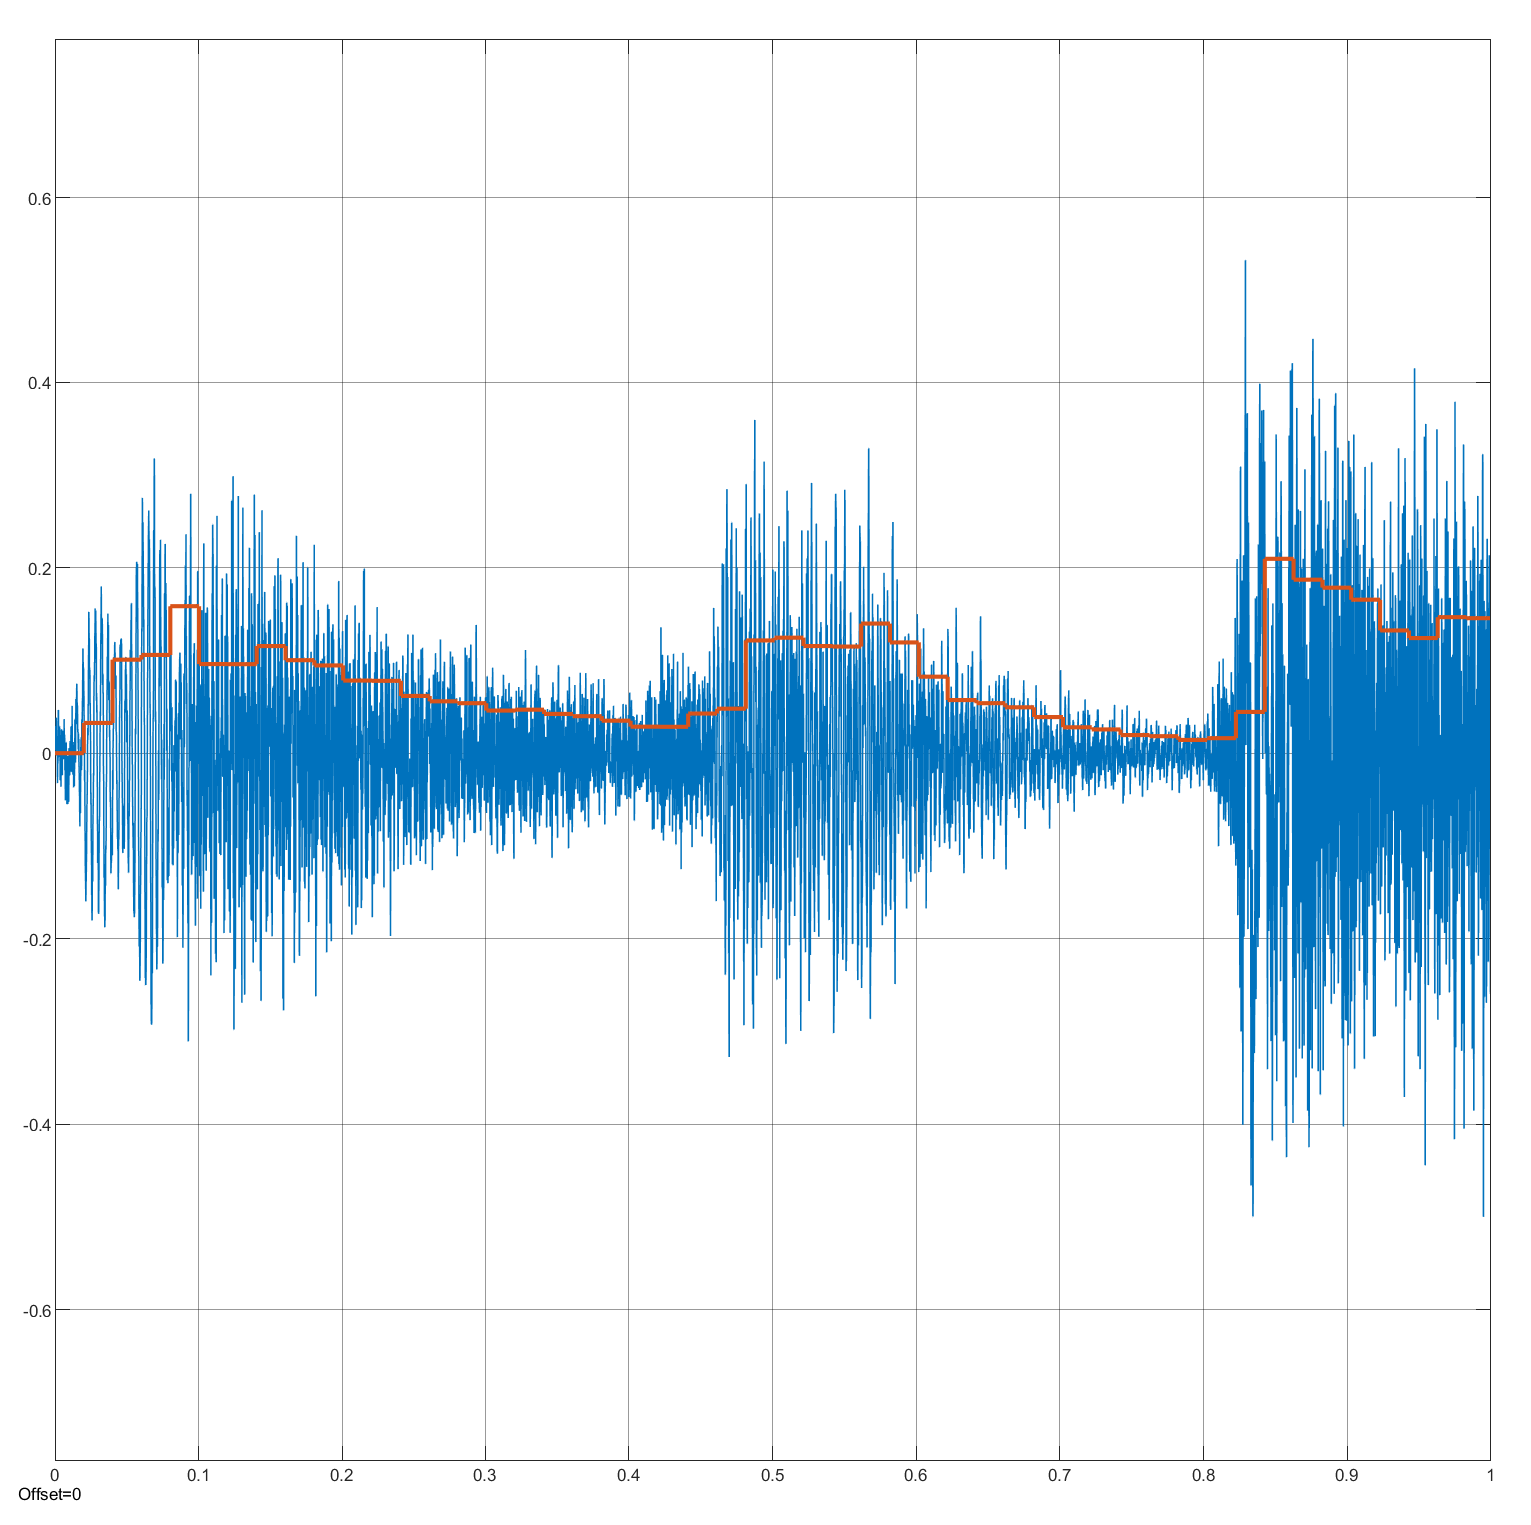
\includegraphics[scale = 0.4]{Figuras/p4_1_envolvente_frame.eps}
    \caption{Resultado de calculo del valor RMS para frames de $20~ms$ al archivo de audio \textit{musica\_16\_16.wav}.}
    \label{envolve}
\end{figure}


\begin{figure}[H]
    \centering
    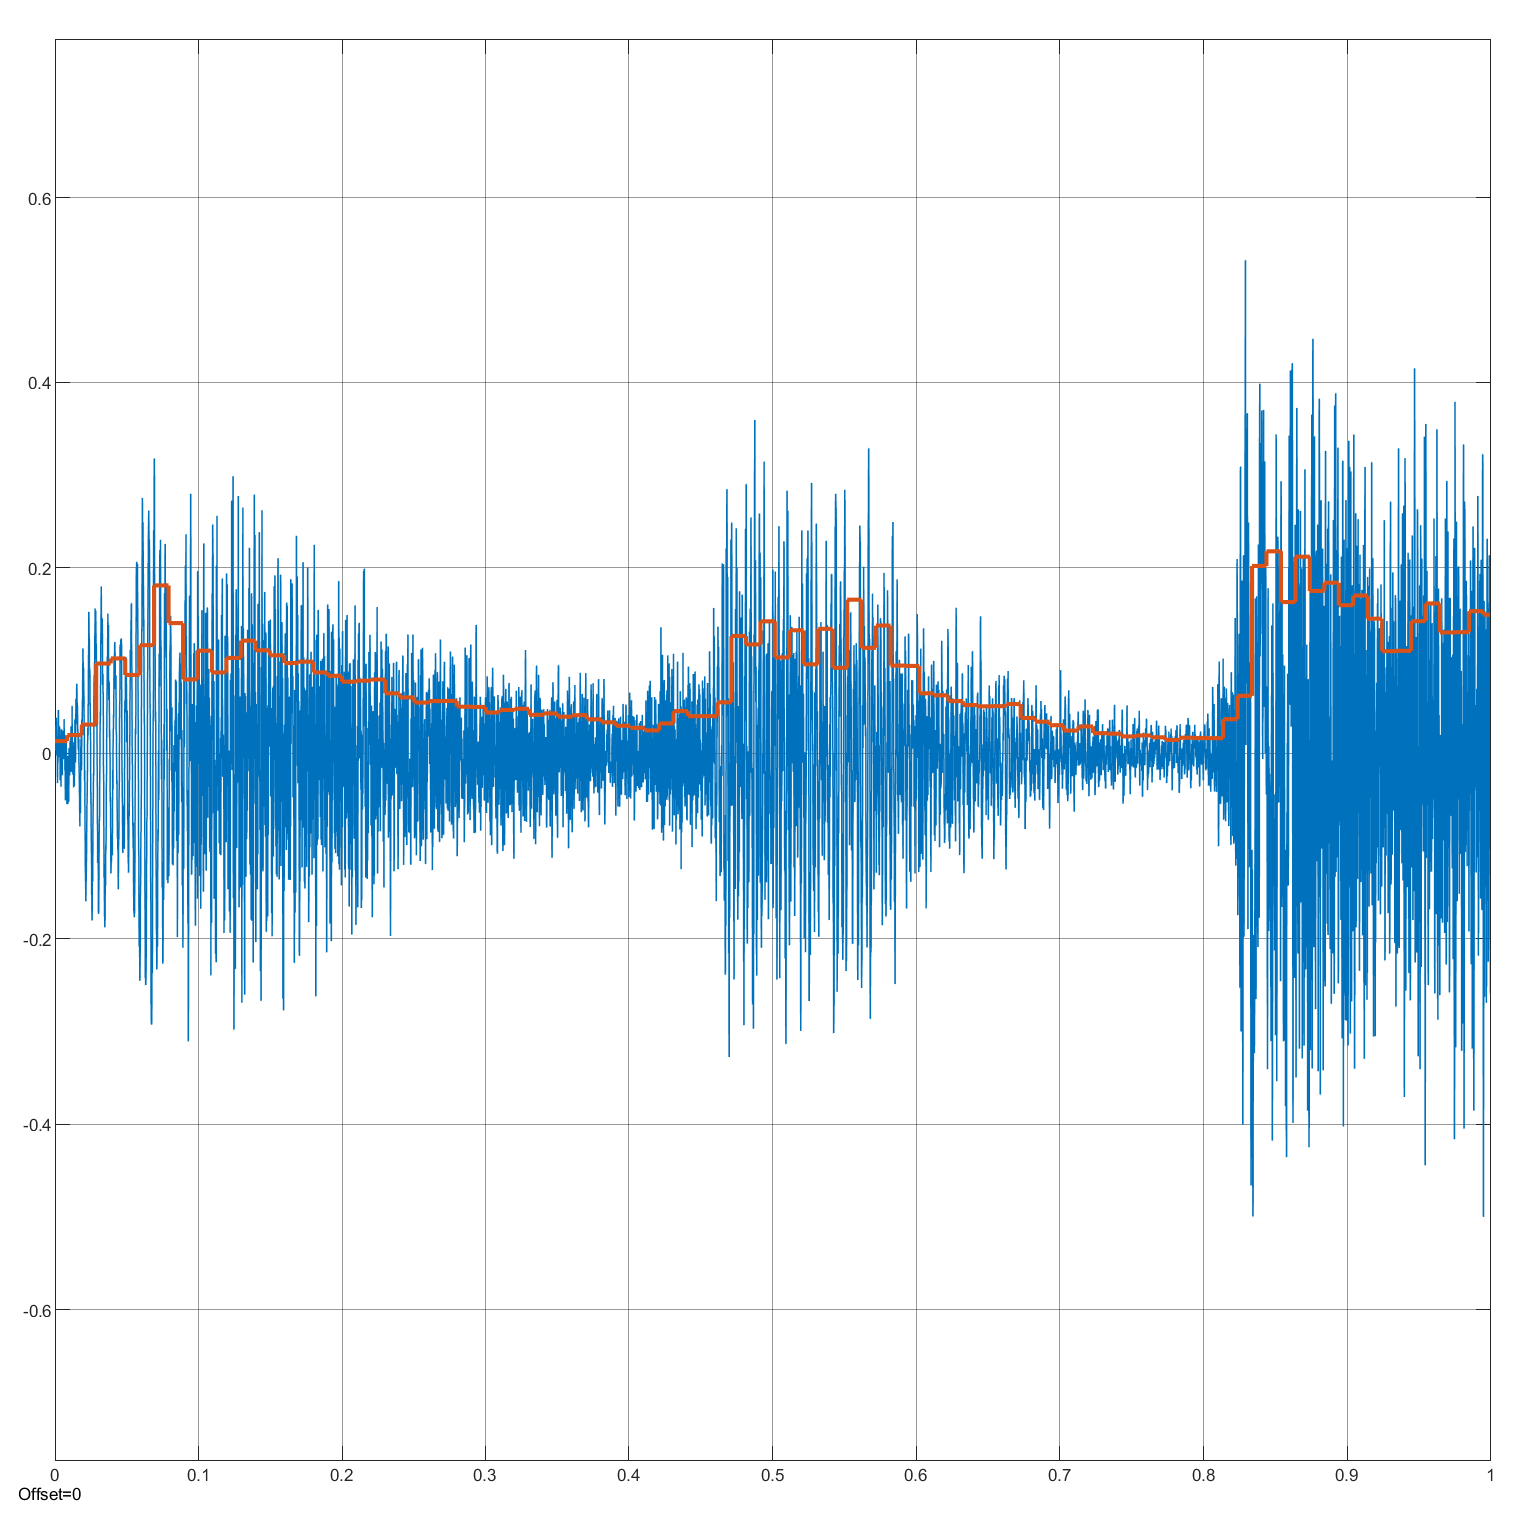
\includegraphics[scale = 0.4]{Figuras/rms_10ms.eps}
    \caption{Resultado de calculo del valor RMS para frames de $10~ms$ al archivo de audio \textit{musica\_16\_16.wav}.}
    \label{envolve10ms}
\end{figure}

\begin{figure}[H]
    \centering
    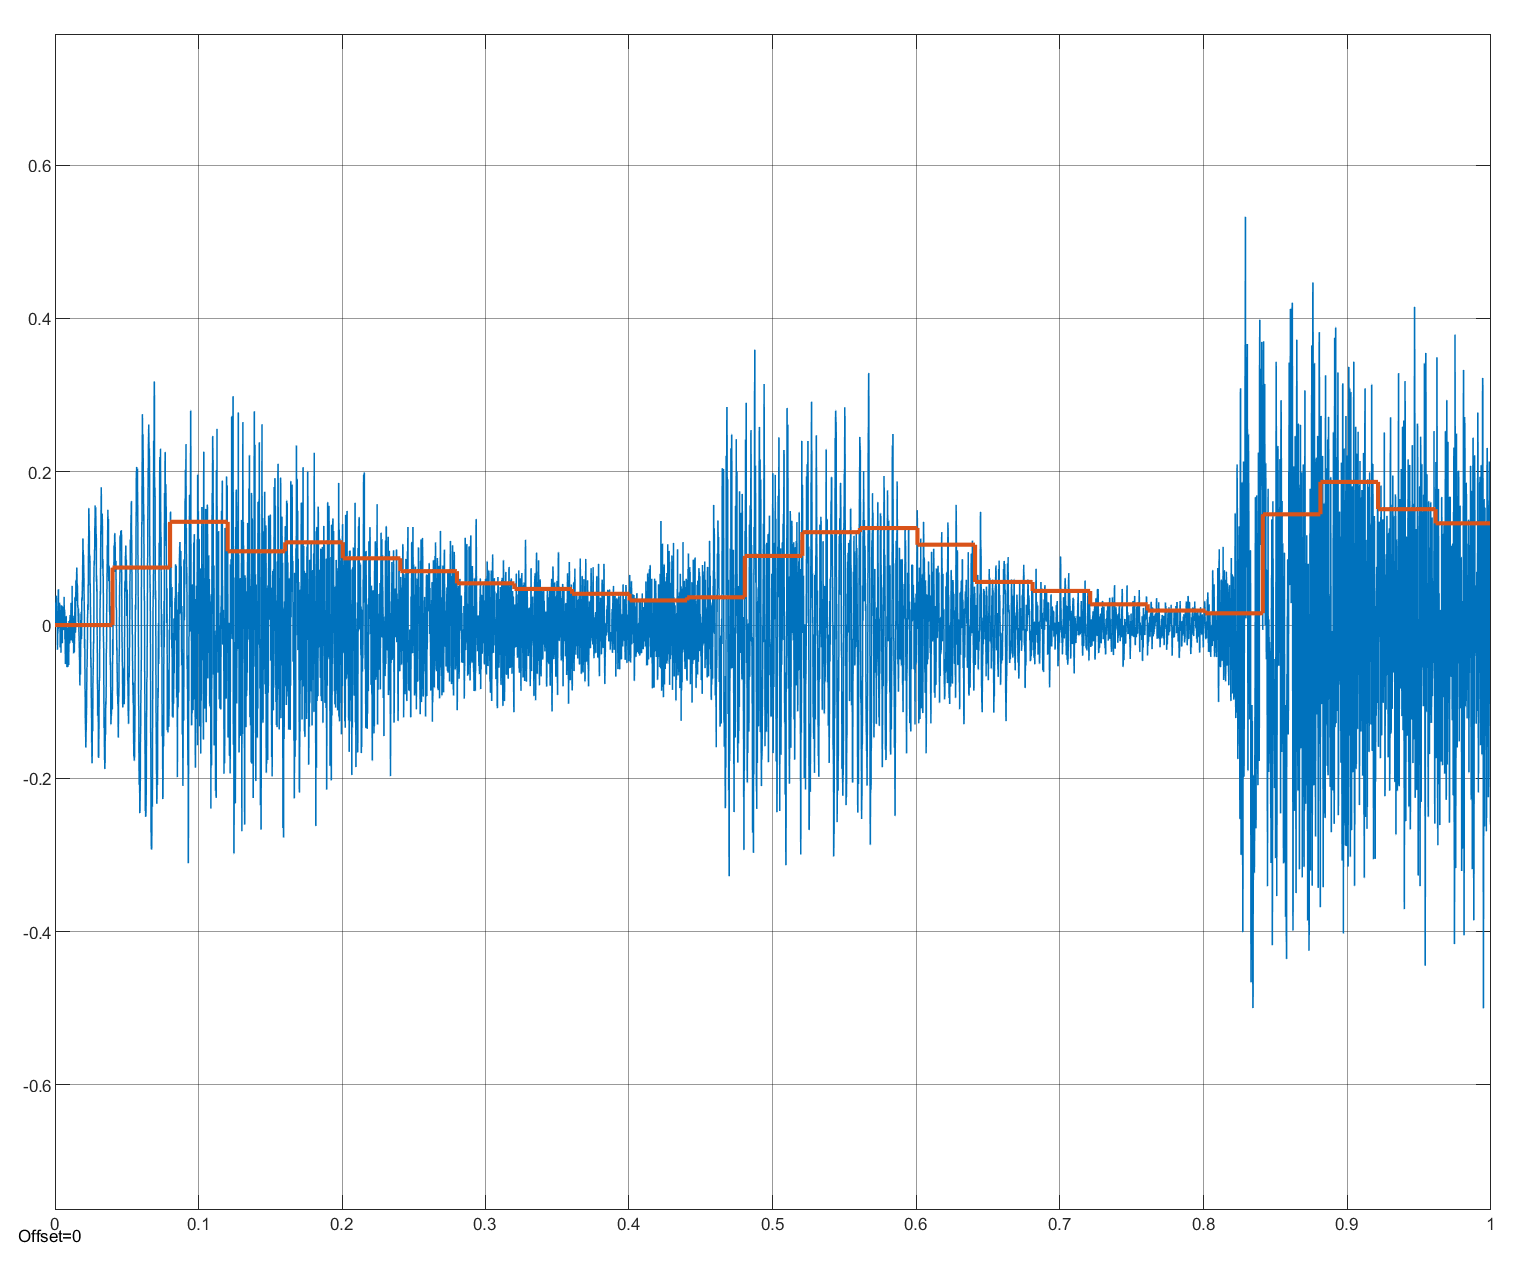
\includegraphics[scale = 0.4]{Figuras/rms40ms.eps}
    \caption{Resultado de calculo del valor RMS para frames de $40~ms$ al archivo de audio \textit{musica\_16\_16.wav}.}
    \label{envolve40ms}
\end{figure}
\clearpage

\section{Resampling: Interpolación y Decimación}
\begin{enumerate}
    \item Se implementa en MATLAB la  función \texttt{y = interpola(x,P)}, que  interpola una señal realizando los pasos de \textit{upsampling} y filtrado. Donde x es la señal de entrada con una frecuencia de muestreo $Fs$ y P es el factor de \textit{upsampling}, es decir el numero de muestras ceros que se agregan a la señal original  entre sus  muestras (Técnicamente se agregan P-1 ceros).
    
    
    \begin{lstlisting}
    function y = interpola(x,P)
        y = [];
        N = length(x);
        
        %Upsampling
        for i = 1:N
            y = horzcat(y, x(i), zeros(1,P-1));
        end
        
        %Filtrado
        B = fir1(40, 1/P);
        
        %Correccion de Magnitud
        y = P*filter(B,1,y);
    
    end
    \end{lstlisting}
    
    Para visualizar el efecto de la interpolación implementada se realizan pruebas con una señal aleatoria de 10 muestras y utilizando un factor P de 7, obteniendo de esta forma las gráficas presentes en la figura \ref{interpola}. Cabe mencionar que por el efecto de el filtro aplicado se genera un retardo de grupo en la señal resultante, este efecto se muestra en la primera gráfica de la figura, mientras que en la segunda gráfica presenta este mismo resultado pero con el resultado de la interpolación eliminando las muestras correspondientes a este   retardo de grupo.
    
    
    
    
\begin{figure}[H]
    \centering
    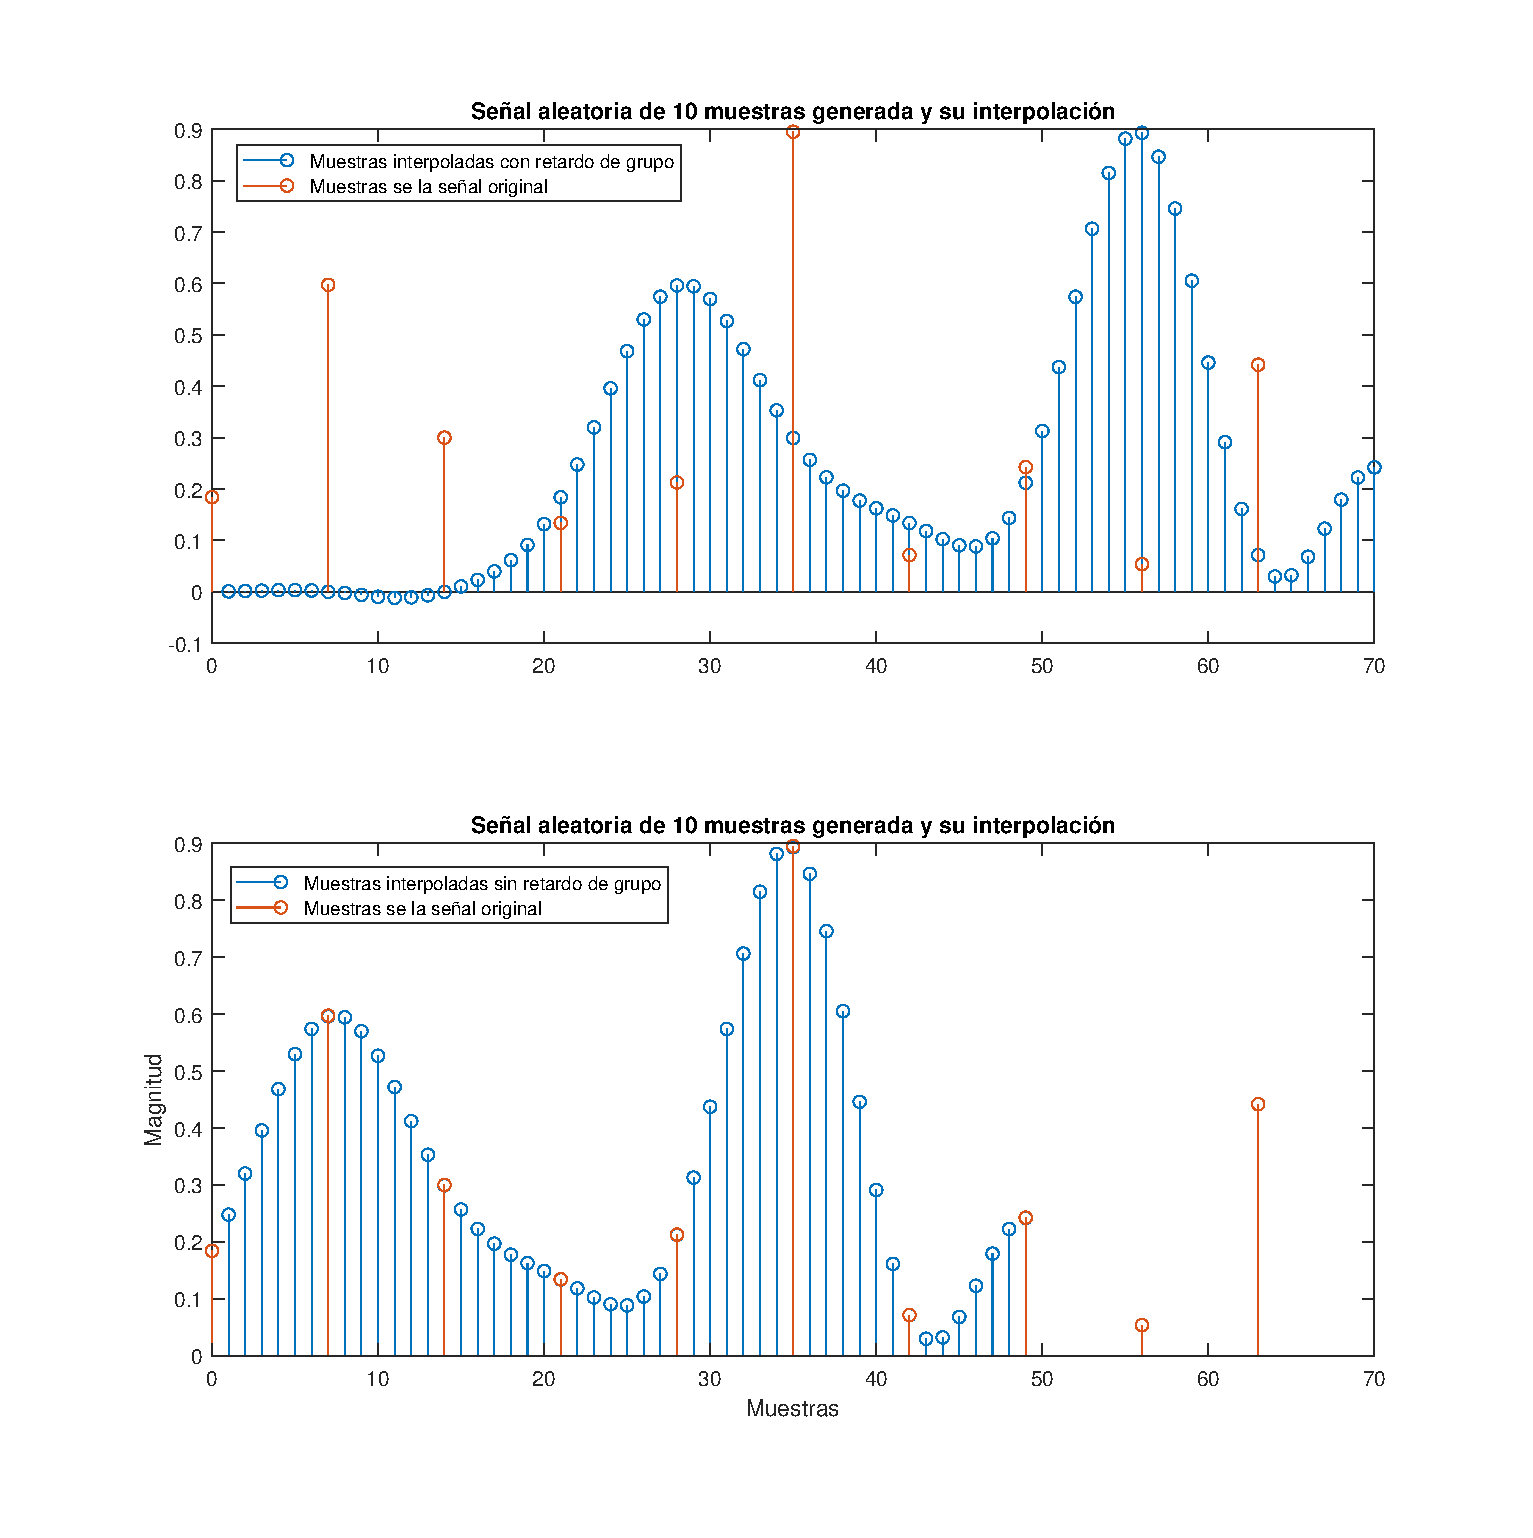
\includegraphics[scale = 0.5]{Figuras/p5_1_interpola.eps}
    \caption{Gráfica de señal aleatoria de 10 muestras junto a su interpolación obtenida.}
    \label{interpola}
\end{figure}
    
    
    Para analizar como va variando el espectro de una señal interpolada  se grafica el espectro obtenido  en  cada paso del proceso de interpolación, esto es, la señal original, la señal luego del \textit{upsampling} y la señal interpolada para el archivo \terxtit{aliasing\_test\_16\_16.mat}. Estas gráficas se muestran en la figura \ref{espectro_inter}, donde se puede ver que el espectro luego del \textit{upsampling} se contrajo  apareciendo la información del espectro a un tercio de la frecuencia a la que aparecía en el espectro de la señal original además de presentar aliases periódicos tal como se  esperaba según la teoría. Finalmente  luego de aplicar el filtro se obtiene el espectro resultante de la  señal interpolada.
    
    
\begin{figure}[H]
    \centering
    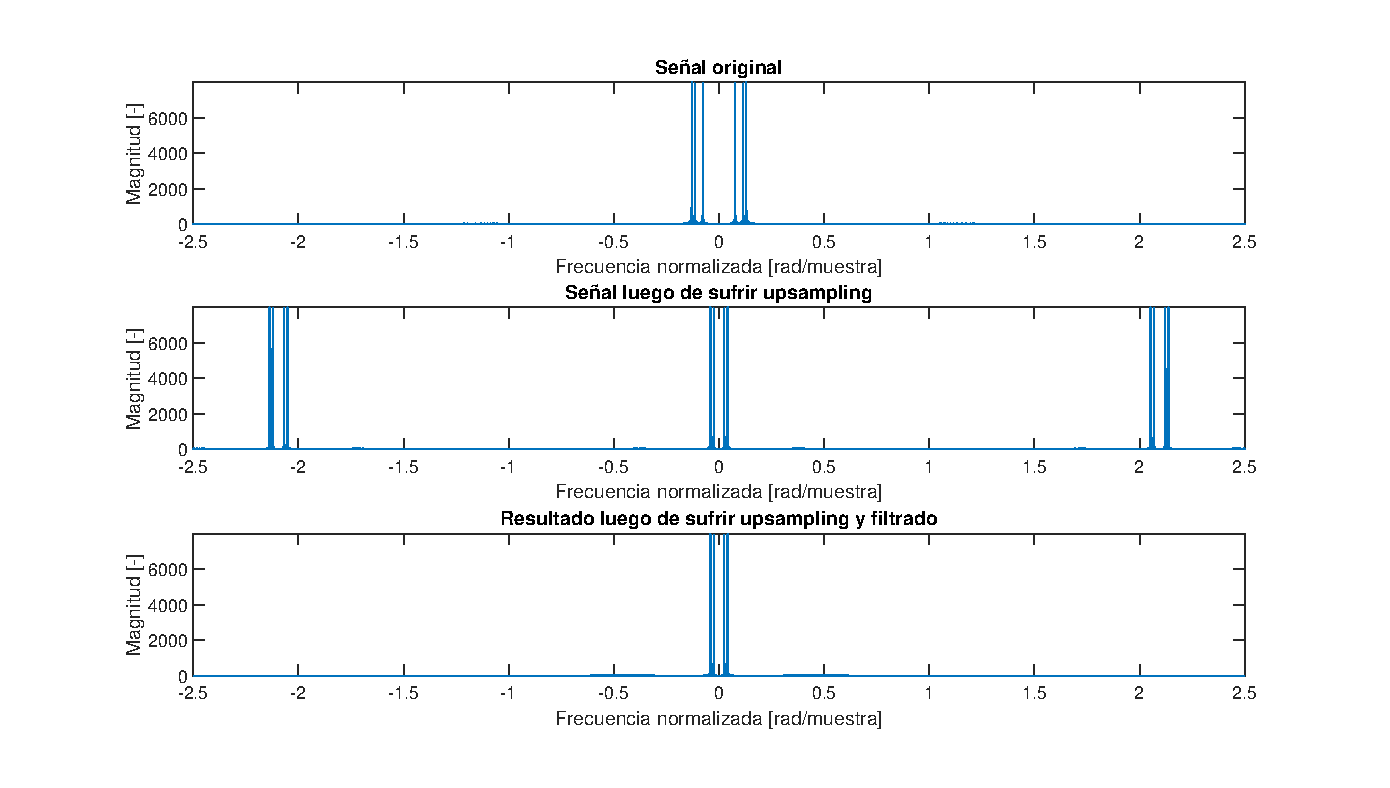
\includegraphics[scale = 0.6]{Figuras/p5_1_espectros.eps}
    \caption{Espectro de los diferentes pasos del proceso de interpolación para el archivo \terxtit{aliasing\_test\_16\_16.mat}}
    \label{espectro_inter}
\end{figure}
    
    
    
Posteriormente se genera una señal Delta de Kronecker en  un vector de muestras donde dicho delta se encuentra en la muestra numero 20,  para poder observar el efecto de la interpolación tanto en muestras anteriores como posteriores al impulso. Esta señal generada se utilizará como entrada al proceso de interpolación que se ha implementado, los resultados obtenidos se muestran en la figura \ref{kroneker}

\begin{figure}[H]
    \centering
    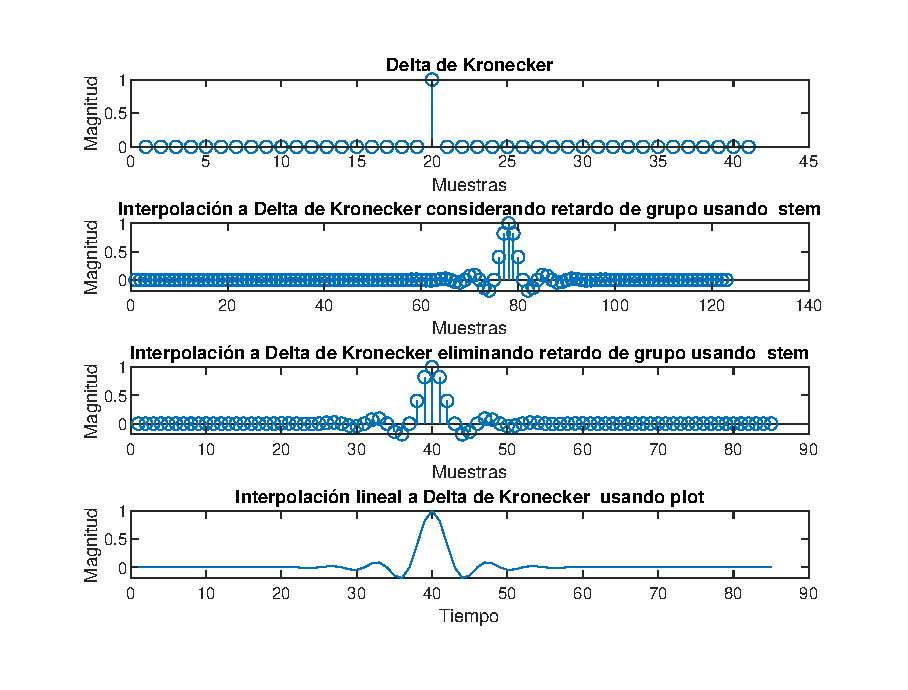
\includegraphics[scale =1]{Figuras/p5_1_kronecker.eps}
    \caption{Interpolación a un Delta de Kronecker.}
    \label{kroneker}
\end{figure}

En la figura anterior se puede ver que la respuesta Y a un impulso de Kronecker se asemeja a una señal \textit{sinc} con el inherente retardo de grupo asociado al filtro (segundo gráfico),ignorando dicho retardo, el resultado  hace sentido, ya que el espectro en frecuencia de un impulso corresponde a una constante que al pasar por un filtro FIR de alto orden (en este caso orden 40), entrega una señal \textit{rect} en frecuencia, al llevar este resultado de vuelta al dominio del temporal se obtiene una teóricamente una señal \textit{sinc}. Se concluye entonces que la respuesta a impulso de  el filtron FIR de orden 40 corresponde a una \terxtit{sinc}.
    
    
    
    
    
\item Se implementa en MATLAB la  función \texttt{y = decima(x,P)}, que  aplica decimación de factor $P$ a la señal de entrada $x$ mediante filtrado y downsampling. La implementación se muestra a continuación:
    
    \begin{lstlisting}
    function Y = decima(X,Q)
        %Filtrado
        B = fir1(40, 1/Q);
        y = filter(B,1,X);        
    
        %Downsampling
        N = round(length(X)/Q);
        Y = zeros(N,1);
        for i = 1:N
            Y(i)= y((i-1)*Q+1);
        end
    
        %Correccion de Magnitud    
        Y = Q*Y;
    end
    \end{lstlisting}

Posteriormente se utiliza la función para procesar la señal \texttt{aliasing\_test} para $Q = 4$ y se grafica la magnitud de la FFT de la señal original y de la señal luego de la decimación. Los gráficos resultantes se muestran en la figura \ref{fig:p5_2}. Se observa el correcto funcionamiento de la función de decimación,  expandiéndose en un factor de $Q$ el ancho del espectro y manteniéndose las amplitudes. 

\begin{figure}[H]
    \centering
    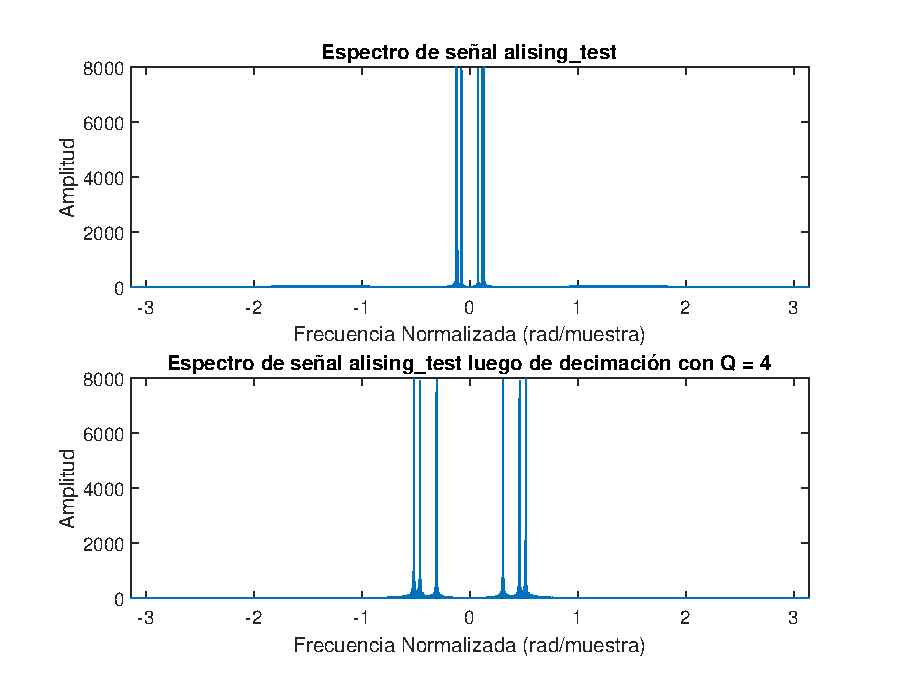
\includegraphics[width = .9\linewidth]{Figuras/p5_2.eps}
    \caption{Espectro de señal \texttt{aliasing\_test} original y luego de aplicar decimación.}
    \label{fig:p5_2}
\end{figure}

\item Se utilizan las funciones de decimación e interpolación para hacer un remuestreo de la señal \texttt{aliasing\_test} desde $16~ksps$ a $12~ksps$.

Para encontrar el factor de decimación se busca llegar a una frecuencia de muestreo que permita llegar a $12~ksps$ usando interpolación. Lo anterior corresponde a encontrar el máximo común divisor entre las frecuencias, por lo tanto el factor de decimación $Q$ está dado por:
$$Q = \dfrac{16k}{\text{M.C.D}(16,12)} = \dfrac{16}{4} = 4 \text{ ksps}$$

Luego el factor $P$ es el necesario para llevar de 4 ksps a 12 ksps, por lo tanto $P = 3$.

Luego se grafica la magnitud de la FFT de la señal original y la señal remuestreada, lo cual se muestra en la figura \ref{fig:p5_3}. Se observa lo esperado en la ''expansión'' del espectro por disminuir la frecuencia de muestreo.

\begin{figure}[H]
    \centering
    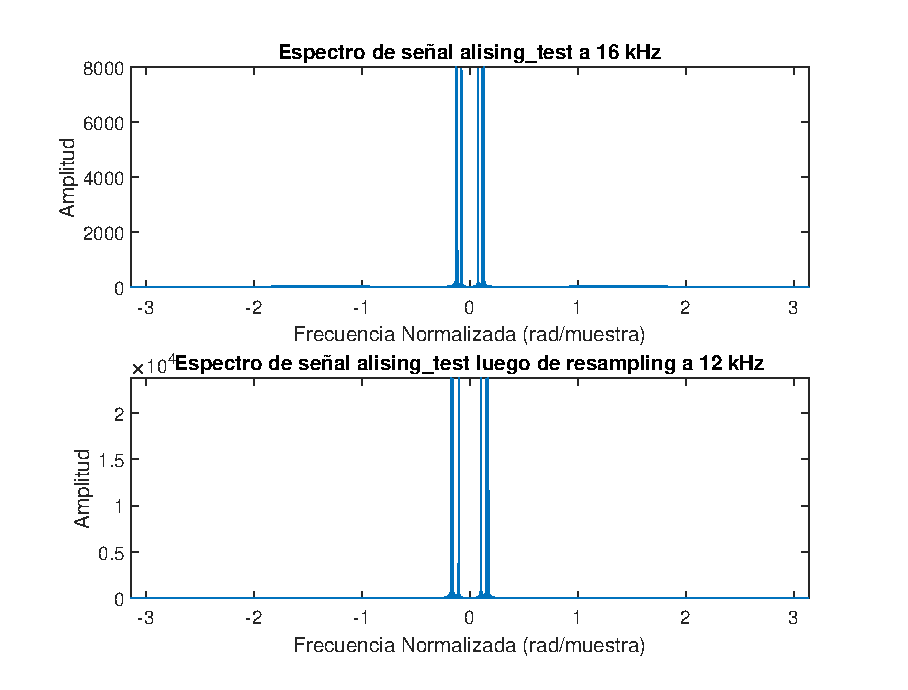
\includegraphics[width = .7 \linewidth]{Figuras/p5_3.eps}    \caption{Espectro de señal \texttt{aliasing\_test} y señal resampleada.}
    \label{fig:p5_3}
\end{figure}

La señal resultante se guarda en el archivo \textit{aliasing\_test\_16\_12.wav} y se adjunta a la entrega.

\end{enumerate}


\clearpage














\end{document}

